In this chapter, we first describe our approach in designing and implementing the Clean Code Analysis Platform. Afterwards, we depict our approach to using machine learning models to detect violations of clean code rules.

\section{Clean Code Analysis Platform}
The goal of the design and implementation of the Clean Code Analysis Platform (CCAP) is a tool for software developers to improve the code quality of existing and new code. The tool accepts a directory containing source code files as input and analyses the input for snippets of improvable code quality. If the analysis classifies a code snippet as problematic, it should help the developer to improve the snippet with information about the problem. Ultimately, this should train the developer to spot problematic code by its own and to write clean code by default, so the number of alerts should decrease over time. At the same time, the overall software quality of a project increases immediately at rewriting a marked snippet and in the long term at training the developer to write code with higher quality.

In order to use the tool effectively, the design and implementation should cover the following requirements:
\begin{description}
    \item[Useability:]  The CCAP should be an easy-to-use tool. Developers shall be able to install and run the tool without difficulties. The extra effort of using this tool should be small, and the developer should use the tool in his day-to-day workflow without additional friction. The developers can interpret the results and localise the issue immediately.
    \item[Extensibility:] The extension of the detectable clean code violations should be easy. A clear defined interface for extensions is required. An extension developer would not need specific knowledge about the internal architecture of the tool. The extensibility allows the desired workflow of a developer finding problematic code in an, e.g. peer-review, formalising it into an extension and sharing this extension with the team. With each iteration, the code quality of all team members would increase.
    \item[Integration:] The tool should be easy to integrate into different systems. These systems include local workflows like git pre-commits or build systems and remote continuous integration/delivery/deployment pipelines.
\end{description}
A more specific requirement is Python as an input and extension language. After JavaScript, Python is the second most popular programming language 2019 according to the Github statistics~\cite{github_inc_state_2019} and the third most popular language according to the TIOBE index (TODO \url{https://www.tiobe.com/tiobe-index/}). Besides the general popularity, Python is heavily used in the scientific community for machine learning and at universities for teaching programming. These groups are part of the potential target audience, and students in particular can benefit from automated reporting of low-quality source code.

\subsection{Architecture}
The CCAP architecture is divided into the main part and two extension possibilities: An extension with analysis plugins adds automated checkers for more rules that are validated by the system. Adding an output plugin allows specifying the output format to fit custom workflow needs.
The main part consists of four components: A core component to act as an orchestration unit, a component for handling the source code input and a component for handling the analysis plugins as well as output plugins. The design follows the requirements and goals for the platform. \Cref{fig:overview_ccap} provides a high-level overview of the components.
\begin{figure}
    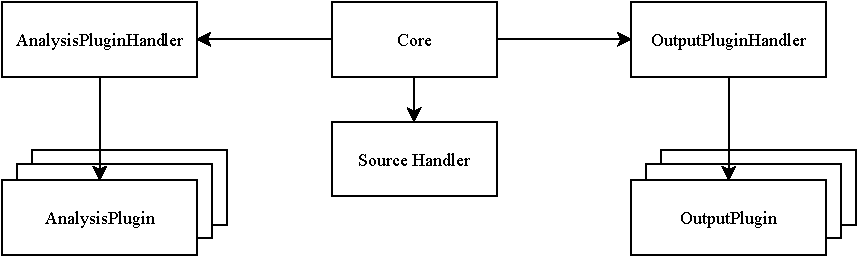
\includegraphics[width=1\textwidth]{img/CCAP/overview_diagram.pdf}
    \caption[High-level schematic overview of the CCAP.]{High-level schematic overview of the CCAP. The core component is the orchestration unit, the source handler parse the source code files and the two plugin handler search for and execute the analysis and output plugins. }
    \label{fig:overview_ccap}
\end{figure}

The core component contains the main function and handles argument validation and parsing. Furthermore, it orchestrates other components by initialising and executing those. This process is divided into the argument parsing, initialisation and execution phase:
In the argument parsing phase, the command line arguments are parsed and validated. It validates the existence of the required input directory argument and the optional plugin path configuration for the analysis plugins and the output plugins. Additionally, the logging level and the output format can be defined. The latter determines, which output plugin will be used, although the existence of the specified plugin is not validated in this phase. A parsing or validation error will cause a program termination without further processing.
The initialisation phase instantiates all components and the analysis plugin handler will scan the specified directories for plugins and keeps an index of all found plugins in memory. The output plugin manager scans for an output plugin, that satisfies the specified argument. If no plugin matches the output argument, the program will terminate and display a failure message to indicate the problem.
In the execution phase, the input handling component scans the input directory for files ending with \texttt{.py} and parses the source code into an Abstract Syntax Tree (AST) per file. In the next step, the core passes the parsed data to the analysis plugin handler. The latter will execute all plugins for all files and collects the results. Afterwards, the core component calls the output plugin component to output the results. If no exceptions occur during the execution phase, the program will be terminated successfully.

The input component scans the given input directory for all Python source code files and parse the source code into an AST. 
For scanning the input directory, an algorithm will walk recursively over all folders and files. The detection of Python source code files is based on the file ending \texttt{.py}. The algorithm will return a list of file paths and the corresponding file content. 
Next, the AST parser is called and will add a parsed AST object to the list besides the file path and content. This list will be passed to the analysis plugins by the analysis plugin handler.  An alternative approach would be to not read and parse the code in the input component, but instead, let the plugins read and parse the file content if needed. With many files to scan, the latter approach would have a lower memory footprint since the file content and the AST will not be held in memory. However, every analysis plugin has to perform an expensive read operation from disk and the performance scales with the number of files and the number of analysis plugins. 
If the input component reads all files, the information is held in the main memory and the performance only scales with the number of files. Since the files are text-based, we expect the number of files needed to exceed the main memory to be high enough to fit most projects.

The analysis plugin handler manages all analysis plugins. This component finds all plugins, executes the plugins and collects the reported results.
During the initialisation phase of the core component, the analysis plugin handler will scan the plugin directory for all Python files. It imports all Python files and scans those for classes, that inherit from an abstract \texttt{AbstractAnalysisPlugin} class. The abstract class defines all methods that need to be implemented in the specific plugin subclass. The analysis plugin handler instantiates all found classes.
During the core execution phase, the core receives a list with the file name, file content and the parsed AST. All plugins are called on a specific entry point method that is defined in \texttt{AbstractAnalysisPlugin} with the aforementioned list. The plugin will return an instance of \texttt{AnalysisReport} with the plugins metadata and a collection of problems. The report is collected for every plugin into a \texttt{FullReport}. Additionally, the report contains information about the overall plugin execution time and run arguments. After all plugins have been executed for all files, the analysis plugin handler returns the \texttt{FullReport} to the core component.

The last component in the execution chain is the output plugin handler that will pass the \texttt{FullReport} to the specified output plugin. It implements the same algorithm as the analysis plugin handler to find all plugins that inherit from \texttt{AbstractOutputPlugin}. Instead of keeping track of all plugins, only the plugin that corresponds to the output format argument is instantiated. The output plugin has an entry point as defined in \texttt{AbstractOutputPlugin}  that is called with all the collected results.

\subsubsection{Analysis Plugins}\label{sec:analysis_plugins}
Analysis plugins provide the easy extensibility of the platform by developers. All users of the tool can extend the set of problems it can detect by implementing a plugin in Python and placing it into the plugin directory of the tool. In order to be compatible with the core components, a plugin has to inherit from the \texttt{AbstractAnalysisPlugin} class. First, the abstract class introduces a class member variable \texttt{metadata} of the class \texttt{PluginMetaData}. A specific plugin class sets this class member in the constructor to provide a plugin name, author and optional website. This metadata is used in the output to show more information about the plugin that reported a problem. Second, \texttt{AbstractAnalysisPlugin} specifies a \texttt{do\_analysis} method as an entry point that the platform will call. It accepts a list of \texttt{ParsedSourceFile} objects that contains the file path, the file content and the corresponding AST for all input files. With this information, the plugin can implement any logic to detect problems. 
For example, the plugin can traverse the AST to look for specific node types, it can use a tokenizer on the content of the files and analyse the token stream or it can run sophisticated machine learning algorithms on the source code.

The plugin can even import third-party libraries, although the user has to install those on the system. After detecting all problems, the plugin returns an \texttt{AnalysisReport}. The report contains the plugins metadata and a list of found problems. 
These problems are instances of a problem class inheriting from \texttt{AbstractAnalysis\-Problem}. The abstract class expects a file path and line number as constructor arguments and requires the plugin developer to override the problem name and description. \Cref{lst:return_none_problem_override} shows an example implementation. The problem name and description will be shown in the final output and should adhere to the following guidelines:

\begin{itemize}
    \item Have a proper name that allows the experienced developer to recognise the problem quickly.
    \item Explain what code construct is problematic.
    \item Give reasons why this code is seen as problematic.
    \item Show guidance and examples on how to fix the problem and improve the code.
\end{itemize}
Although it is possible to use one plugin for multiple, different problem types, having one plugin for one problem type helps to reuse and share the plugin. Additionally, it can be disabled easily by removing the plugin from the plugin folder and complies to the Single-Responsibility Rule.


\begin{lstlisting}[language=Python, label=lst:return_none_problem_override, caption={Example for overwriting the \texttt{AbstractAnalysisProblem} with a specific implementation. The problem name and description are overwritten.}]
    class ReturnNoneProblem(AbstractAnalysisProblem):
        def __init__(self, file_path, line_number):
            self.name = "Returned None"
            self.description = "Returning None is dangerous since the caller has to check for None. Otherwise, a runtime exception may occur."
            super().__init__(file_path, line_number)
    \end{lstlisting}
    
\paragraph{Steps to create an analysis plugin}
In order to extend the CCAP with an analysis plugin, the following steps are required for a developer:
\begin{enumerate}
    \item Create a \texttt{.py} file with a class inheriting from \texttt{AbstractAnalysisPlugin}.
    \item Instanziate \texttt{PluginMetaData} and assign it to the metadata member.
    \item Define a problem class inheriting from \texttt{AbstractAnalysisProblem} and set the problem name and description following the guidelines above.
    \item Implement the \texttt{do\_analysis} method with a \texttt{ParsedSourceFile} parameter. Return an \texttt{AnalysisReport} instance with all found problems.
    \item Place the \texttt{.py} file into the analysis plugin directory of the tool.
\end{enumerate}
While these are the minimum required steps to implement the plugin, the developer is free to add additional methods, classes or import libraries as necessary.
Furthermore, it is advisable to implement several tests to ensure the plugins correctness. CCAP uses the pytest\footnote{\url{https://docs.pytest.org/en/stable/}} library for testing. Implementing a test is as easy as writing a function with a \enquote{test\_} prefix and running the \texttt{pytest} command. The plugin can be tested by simulating a call from the CCAP core with a mocked \texttt{ParsedSourceFile}. 

\subsection{Return None Plugin}\label{sec:return_none_ccap_implementation}
A rather simple analysis plugin demonstrates the capabilities of the CCAP: The Return None Plugin scans the source code for functions that return the \texttt{None} value. Returning texttt{None} may result in runtime exceptions if the function caller does not expect and handle a potential \texttt{None} return. Although \texttt{None} can be returned directly or as a value of the returning variable, this plugin only focus on the explicit \texttt{return None} statement to showcase the options for the developer to analyse the source code. We will later refer to this problem type as \texttt{RETURN\_NONE} (RN).

Detecting a \texttt{return None} statement is possible in multiple ways. The following shows the possibilities for a developer to implement such a detector:
\begin{description}
    \item[Regular Expression:] In the \texttt{do\_analysis} method, a developer has access to the source code as a string. Therefore, it is straightforward to use a regular expression to detect a \texttt{return None} statement:
    \begin{lstlisting}[language=Python]
import re
matches = re.finditer(r"return None", source_file.content, re.MULTILINE | re.DOTALL) \end{lstlisting}
    Since the regex library only returns the start and end index of matches, these have to be converted to line numbers. Afterwards a \texttt{ReturnNOneProblem} instance can be created for every match and added to the \texttt{AnalysisReport} for this plugin.

    This approach uses regular expressions to match patterns in a string without utilising the structures of the code. It is a simple but powerful way and most developers are familiar with regular expressions. On the flip-side, source code may have various syntactic ways to express a semantic. Consequently, the regular expressions have to be designed carefully to cover all variations. For instance, it is possible to encounter a doubled whitespace, that would break the aforementioned regular expression. Additionally, regular expressions do not operate on the structure of the code; therefore, they can not detect high-level patterns on the code structure.
    \item[Tokenization:] The process of dividing a character stream into a sequence of tokens is called tokenization (also known as lexical analysis). With the Python tokenizer, a token can contain multiple characters and has a token type like name, operator or indentation. A token sequence provides more information about the code structure that can be used to detect problematic patterns. 
    A token sequence for a \texttt{return None} statement would be the following: 
    \begin{lstlisting}[language=Python]
[...(type: "NAME", value: "return"), (type: "NAME", value: "None")...]\end{lstlisting}
    A simple algorithm would scan the sequence for two subsequent name tokens with the values \texttt{return} and \texttt{None}. The abstraction level of a token sequence is higher than of a character sequence. Since the whitespace between \texttt{return} and \texttt{None} provides no semantic meaning, it is removed on this abstraction level. The regular expression-based approach would have to deal with problems as the doubled whitespace. In contrast, the token-based approach profits from the higher abstraction level and can access meaningful tokens directly.
    \item[Abstract Syntax Tree]: After tokenization, a parser takes the token stream and parses it into a hierarchical data structure like an Abstract Syntax Tree (AST). With an AST, the code is represented structurally and it is possible to traverse the tree following the structure of the code. The AST consists of nodes with different types and children. For instance, a node represents an \texttt{if} expression and has a \texttt{test}, \texttt{body} and \texttt{orelse} children. It is possible to access the condition (\texttt{test} children) and the body of the if statement as descendant nodes in the AST. Analysing an AST allows a higher abstraction level then analysing the token string since the AST represents the code structure. Therefore, automated checkers for more abstract rules that analyse the code structure are possible.

    To detect a \texttt{return None} statement in the abstract syntax tree, an algorithm would traverse all AST nodes looking for a return-typed node. If found, the \texttt{value} descendant contains the expression after the \texttt{return} keyword. A \texttt{None} value would be represented as a node of type \texttt{Constant} or \texttt{NameConstant}, depending on the parser version. The \texttt{value} descendant of the node may then be checked for equality to \texttt{None}. All AST nodes contain the corresponding line number that is necessary for creating a problem message. See \Cref{lst:return_none_detection_algorithm} for a Python implementation. 


    Analysing the AST works best to find problems in the code structure since the AST represents the code structure in a well-defined, traversable data structure. Although simpler patterns like the \texttt{return None} could be detected using regular expressions, a detection on AST level allows detecting the semantic meaning instead of the syntactic representation of a problem. For more complex problems, it is inevitable to use the AST most of the time.
\end{description}

\begin{lstlisting}[float,floatplacement=h, language=Python, label=lst:return_none_detection_algorithm, caption={Detecting a \texttt{return None} by analsing the AST data structure.}]
for node in ast.walk(a.ast):
    if isinstance(node, ast.Return):
        return_value = node.value
        if isinstance(return_value, ast.Constant) or isinstance(return_value, ast.NameConstant):
            if return_value.value is None:
                problems.append(ReturnNullProblem(a.file_path, return_value.lineno))\end{lstlisting}


This implementation covers only the simple case, in which \texttt{return None} is written explicitly. Of course, several variations are possible, that would not be detected by this plugin and would require more sophisticated algorithms. Evaluating, if machine learning models trained on this simple rule can also detect such modifications is part of \hyperref[rq:3]{RQ3}.

Since detection alone is not a great help for the user, a useful description of the problem is necessary. 
As described in \Cref{sec:background:returning_none_and_error_handling}, there are some alternatives to returning none. If returning \texttt{None} indicates an error, it is better to raise an exception and provoke an explicit error handling in order to prevent runtime errors. If the standard return type is a collection, an empty list is more appropriate, since the function caller will most likely write the logic for an unknown amount of list items. However, if the standard return type is a single object, it is not apparent what to return. With PEP484, an optional type was introduced as a type hint in Python 3.5~\cite{van2014pep}. A static type checker for Python like mypy outputs a warning if a developer forgets to check an optional for not being \texttt{None}~\cite{lehtosalomypy}. 

\paragraph{Condition with Comparison}\label{sec:condition_comparison}
The second plugin detects a direct comparison in a conditional statement. For better readability and understandability, the clean code rules suggest to use a function call with an appropriate name that evaluates to \texttt{true} or \texttt{false}. This function call allows a natural reading of the conditional statement without deciphering the meaning of the boolean logic.

An if-statement consists of a condition, a body and an else part. If the condition evaluates to \texttt{true}, the body is executed. Otherwise, the else part is executed. Any logical expression or a function call will be evaluated in the condition. A simple algorithm to detect a comparison in the condition would take the AST, search for \texttt{if} nodes, and check if the condition part is a compare node.
However, the simple algorithm would not detect a negation and logic AND/OR conjunction. Consequently, a recursive algorithm has to follow logic operators and checks the expressions for comparison nodes. The simple approach does not provide value for the CCAP, but we use if for the machine learning evaluation. We later refer to the code detected with this algorithm as \texttt{CONDITION\_COMPARISON\_SIMPLE}.

Following these considerations, an advanced algorithm would scan for \texttt{if} nodes in the AST. The conditional part as a boolean expression is evaluated in a recursive. It can be a boolean operation (like AND/OR) or a unary operator (like NOT). In these cases, the function will be called recursively with the respective expressions. If the conditional part is neither a boolean operation nor a unary operator, the function returns \texttt{true} if a single expression is not a function or method call. The clean code rules recommend a function or method call instead of a comparison to maintain readability. 
The last case would be the base case in the recursion. \Cref{lst:condition_coparison} shows the Python implementation of this algorithm and the detected code patterns. We will later refer to the problem type of this advanced algorithm as \texttt{CONDITION\_COMPARISON} (CC). 
\begin{lstlisting}[float, floatplacement=h, language=Python, label=lst:condition_coparison, caption={Recursive function to analyse an if statement for direct comparisons. Since a condition should contain a method call, the function returns False if this is not the case.}]
def _check_if_direct_comparison(self, node):
    if isinstance(node, ast.BoolOp):
        violated = False
        #check all expressions of the boolean operator
        for value in node.values:
            if self._check_if_direct_comparison(value):
                violated = True
        return violated
    elif isinstance(node, ast.UnaryOp):
        return self._check_if_direct_comparison(node.operand)

    return not isinstance(node, ast.Call)\end{lstlisting}

\subsubsection{Output Plugins}
With output plugins, CCAP adds additional flexibility towards the output format. Depending on environmental requirements, the output can be adapted with custom logic by defining an output plugin. For instance, running the tool locally could write the results to the standard output in a human-readable way or create a formatted HTML file to be displayed in the browser. A machine-readable JSON output may be preferred when running inside an automated workflow.

Output plugins follow similar concepts as analysis plugins. A plugin class inherits from \texttt{AbstractOutputPlugin}. The abstract class introduces the metadata member of the \texttt{PluginMetaData} class to encapsulate plugin name and author information. Additionally, a second member variable \texttt{output\_format} has to be defined with a short abbreviation for the output format. This field is used by the output plugin handler to select the output plugin by the run arguments. It should be globally unique, or the first found plugin will precede other plugins with equal naming. We suggest using a custom prefix to the format name to maintain global uniqueness.

As an entry point, the method \texttt{handle\_report} has to be implemented. The method provides an instance of \textit{FullReport} as its argument. The \texttt{report} field holds a collection of \texttt{AnalysisReport} for every analysis plugin that was executed. With metadata and problem information, the output plugin has access to all required information to produce the desired output.

\paragraph{Steps to create an output plugin}
To extend the output capabilities of the CCAP, the following steps are, similiar to analysis plugins, required:
\begin{enumerate}
    \item Create a \texttt{.py} file with a class inheriting from \texttt{AbstractOutputPlugin}.
    \item Instanziate \texttt{PluginMetaData} and assign it to the metadata member.
    \item Set the \texttt{output\_format} field with a unique abbreviation for this output format. Since it should be unique, a custom prefix prevents a name collision with preexisting plugins.
    \item Implement the \texttt{handle\_report} method with a \texttt{ParsedSourceFile} parameter. 
    \item Place the \texttt{.py} file into the output plugin directory of the tool.
\end{enumerate}

\paragraph{Standard Output Plugin}
The Standard Output Plugin writes the formatted output to the \texttt{stdout} stream. It is enabled by default if no output plugin is explicitly specified. 

The output is divided into a general part and the problem list. The former contains the input path, all executed plugins, and a summary field with the number of problems in total. The latter displays the list with problems, grouped by analysis plugin.  
For each problem, the problem name, file path, line number and description is printed. A colon separates the file path and line number. Some terminals parse the path and line number so that a user can click the path and it opens the default editor with the cursor in the correct line. A sample output is printed in \Cref{lst:stdout}.

\begin{lstlisting}[float, floatplacement=h, label=lst:stdout, caption={Example output to \texttt{stdout} of the Standard Output Plugin. Besides a list of problems, it also outputs additional }]
Analysis Report on /Users/enrico/MA_CleanCodeAnalyser/test_programs.
Analyse Plugins: Condition Method Call Plugin, Simple Condition Method Call Plugin, Return None (Null) Plugin, Sample Plugin.
Summary: Found 16 problem(s)
    ----------------------------------------
PROBLEMS:
    PLUGIN NAME: Condition Method Call Plugin by Enrico Kaack <e.kaack@live.de>
        Found: Explicit comparison in condition in /Users/enrico/MA_CleanCodeAnalyser/test_programs/return_none.py:18
            Explicit comparisons in conditions should be replaced by method call for better readability
...
PLUGIN NAME: Return None (Null) Plugin by Enrico Kaack <e.kaack@live.de>
        Found: Returned None in /Users/enrico/MA_CleanCodeAnalyser/test_programs/return_none.py:4
            Returning None is dangerous since the caller has to check for None. Otherwise, a runtime exception may occur.
\end{lstlisting} 

\paragraph{HTML Output Plugin}
For larger projects, the Standard Output Plugin may not be sufficient to get an overview of the project or to generate a report. Therefore, the HTML Output Plugin creates a \texttt{report.html} file that can be opened in every browser. The report provides a cleaner overview and the scrolling capabilities of a browser. It has similar general data at the top as the Standard Output Plugin, but it moves the problem description into a tooltip to offer a more compact overview. See \Cref{fig:screen_html_output} for an example screenshot.

\begin{figure}
    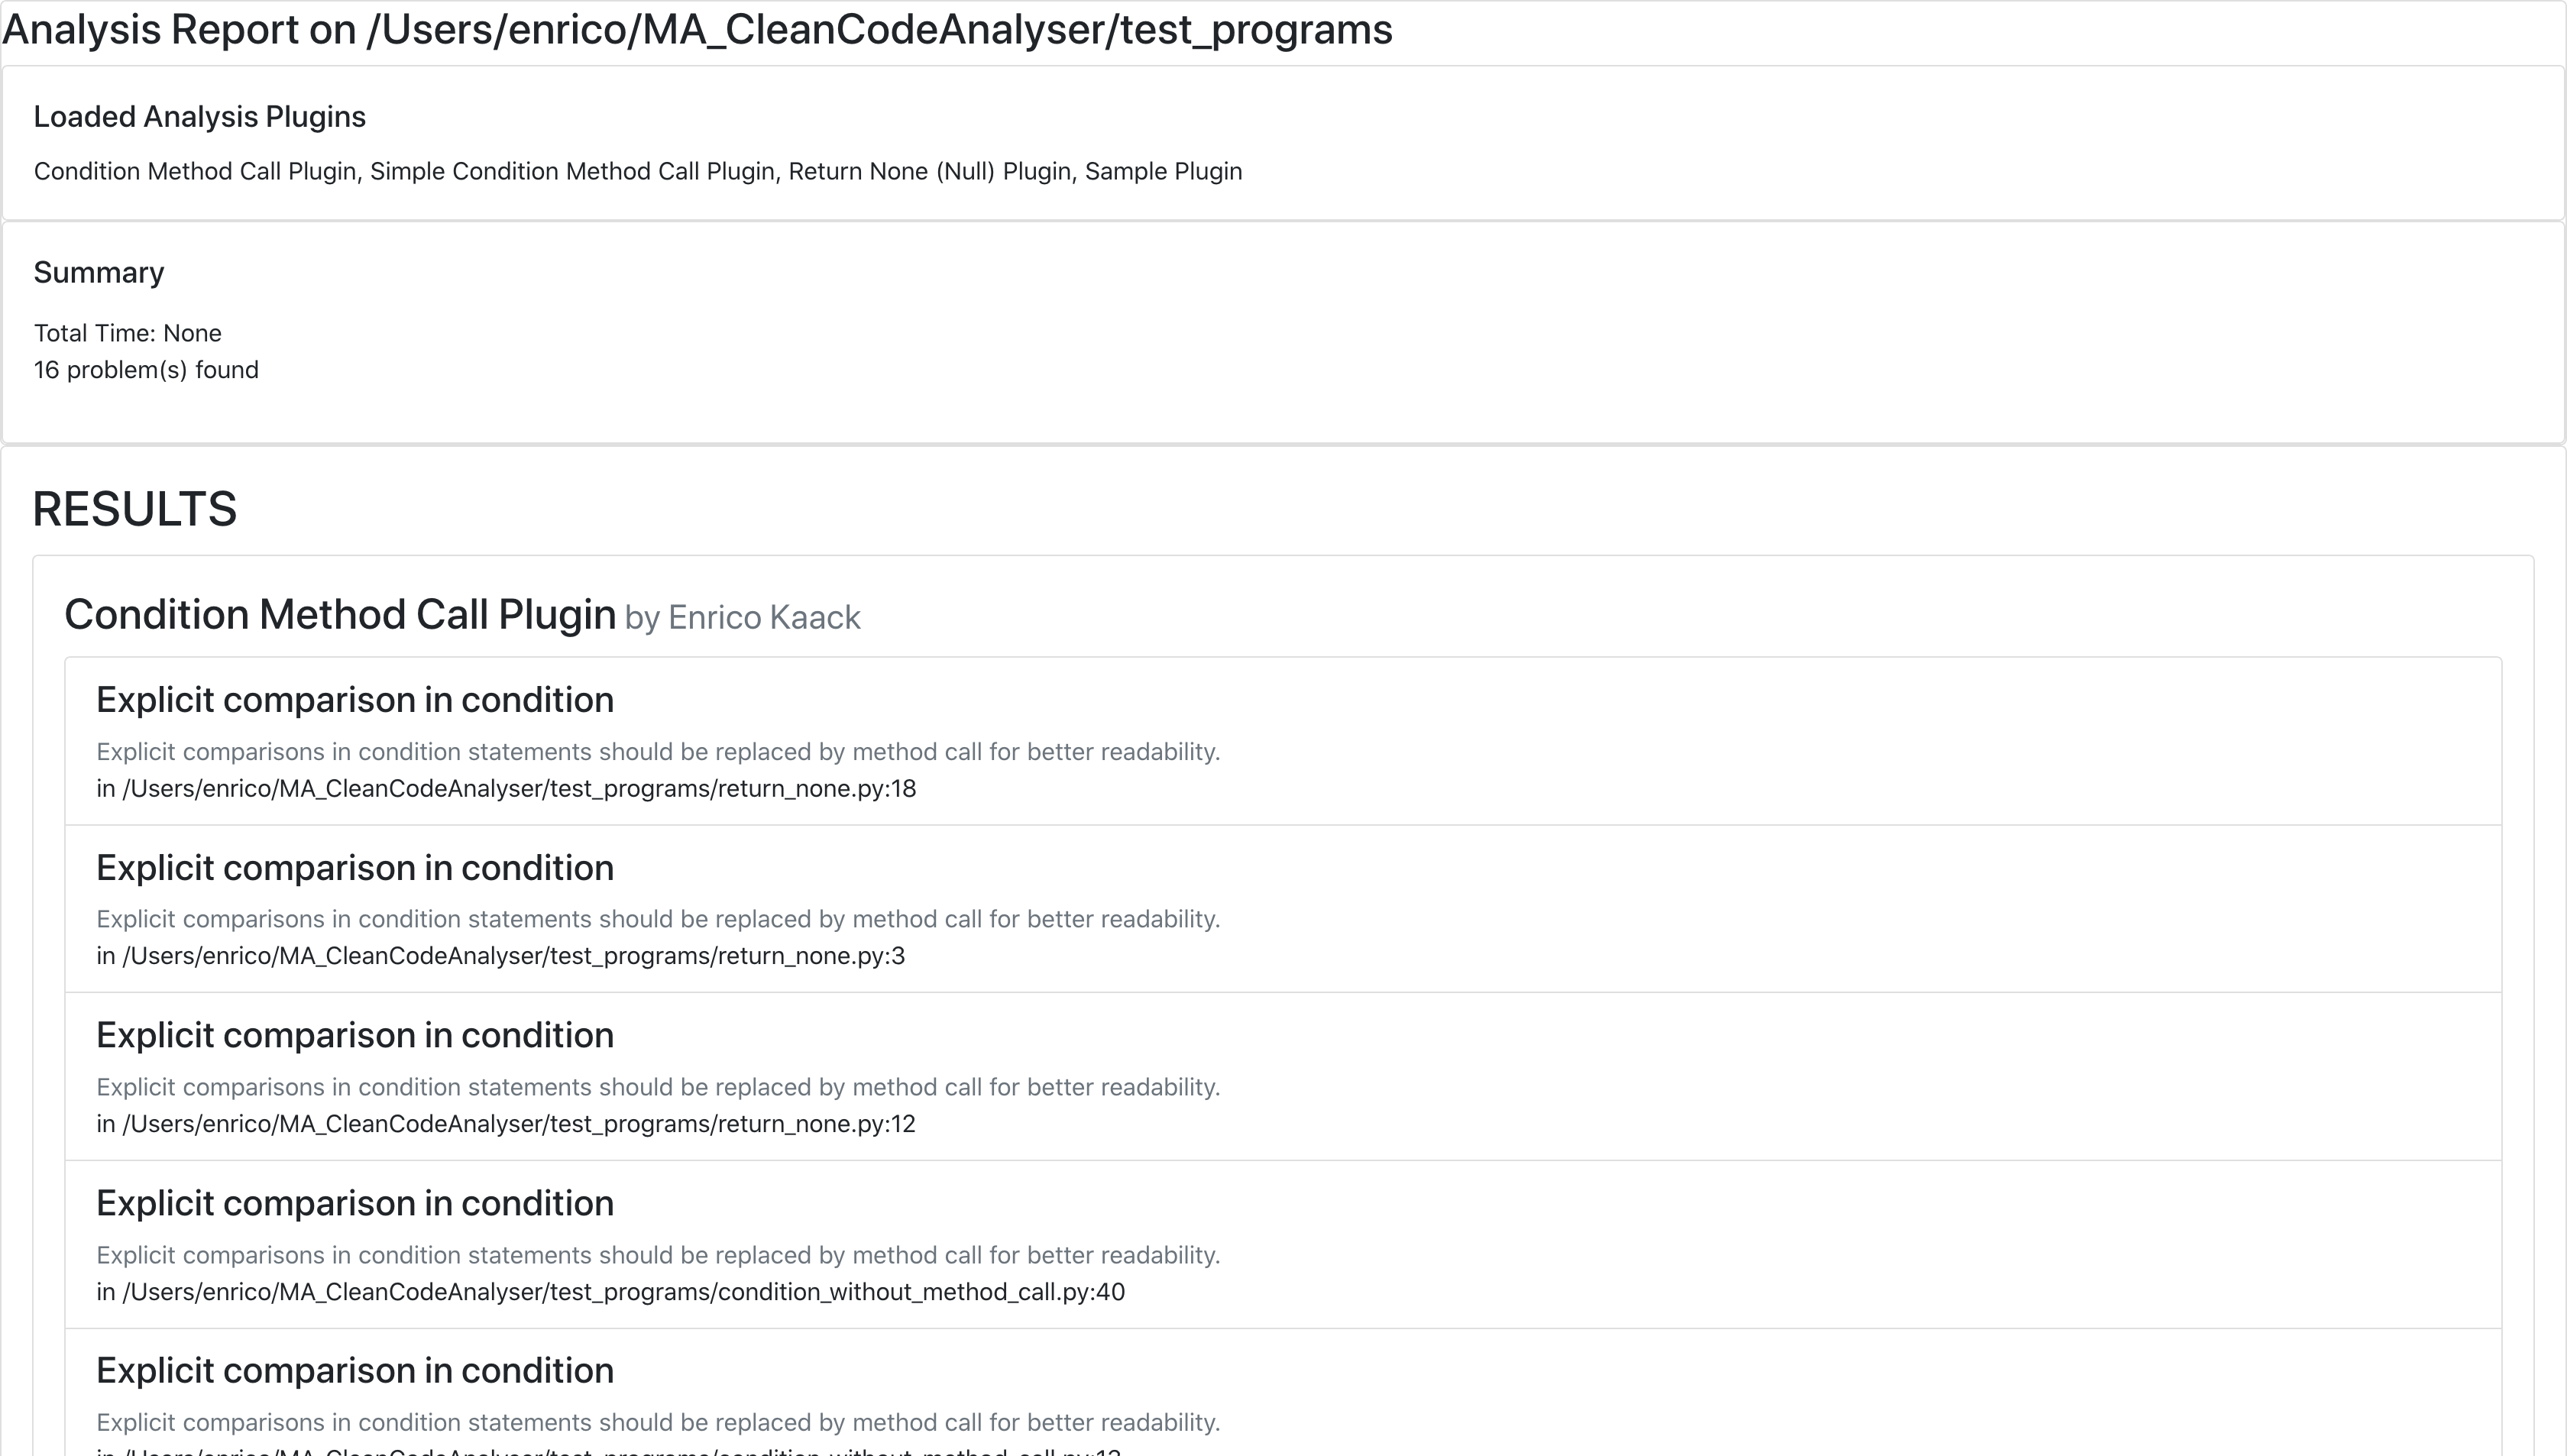
\includegraphics[width=1\textwidth]{img/CCAP/screenshot_html_output.png}
    \caption{Output of the HTML Output Plugin, displayed in a browser.}
    \label{fig:screen_html_output}
\end{figure}

\subsection{Improvements}
While the core functionality exists, extensions for the CCAP would aim for improved useability. One crucial improvement in useability would be an IDE integration for common IDEs like Visual Studio Code. A good starting point would be the Language Server Protocol\footnote{\url{https://microsoft.github.io/language-server-protocol/}}. This IDE integration requires a language client as a Visual Studio Code extension and a protocol-compliant language server. The latter would wrap the CCAP and modify it slightly to process a single, changed document and return the results. Since the CCAP architecture is modular, this should be possible without larger modifications. 

Another feature would be a configuration to disable specific analysis plugins for a project. With the current architecture, this would be possible by moving the analysis plugin file outside the plugin directory. A configuration with command-line parameters or with a hidden config file per project would have a better user experience. The latter could also be committed to the version control system, so every team member has the same configuration.

Continuing on configuration possibilities, having configuration possibilities for plugins would increase the flexibility for a plugin developer. Introducing configurable warn levels like \texttt{warning} or \texttt{error} could help in continuous integration pipelines to decide if a build succeeds with warnings or if a build should fail because of error-level problems. Some rule violation could be seen as recommendations to improve (warning level), whereas other violations may be unacceptable (error level).

Last, a feature to disable problem reporting for a specific code location could bring a boost in user acceptance. While some clean code rules are objective and can be measured precisely, some rules may not apply to every occurrence of the situation. For instance, the clean code guidelines generally suggest not to have more than three function arguments; it may be necessary or even inevitable to have four arguments. The CCAP would report this as a problem, but the user should be able to decide if it is acceptable. In this case, the problem type on this specific location should not be reported in the future. In the current version, the user has no way to ignore a specific problem. Consequently, the number of problems the user has to ignore will accumulate over time until the user abandons the tool since it does not provide an added value over the frustration of manually ignoring problems.

\section{Clean Code Classification}\label{chap:clean_code_classification}
In the previous chapter, we presented a platform to check for clean code rules. This platform requires analysis plugins to detect specific problems. These handwritten rules work well for rules with a basic level of complexity. However, certain rules of an advanced level of complexity may require a complicated analysis of the AST, the data-flow or the inter-module dependencies. Furthermore, rules with a high level of complexity can be subjective, and we do not see a way of detecting those rule violations with a deterministic algorithm.

Therefore, this chapter introduces an approach to evaluate different supervised machine learning models to classify code into clean code or problematic code. Furthermore, we describe how we modify the code to test the generalisation capabilities of the models. The mentioned machine learning models include random forest classifier, support vector machines, gradient boosting classifier and a recurrent neural network model based on Long Short Term Memory units. 

The objectives are twofold: For \hyperref[rq:2]{RQ2}, we train, evaluate and compare the different models on the detection of different code violations. Then we manipulate the source code to test in \hyperref[rq:3]{RQ3}, how well the models generalise to non-seen variations of the rule violations.

To achieve our objectives, we will train our models on the dection of three problem types: 
\begin{enumerate}
    \item The \texttt{RETURN\_NONE} (RN) problem type covers a \texttt{return None} statement in Python code (see \Cref{sec:return_none_ccap_implementation}). A detector would report such a statement as this problem type.
    \item A detector for the \texttt{CONDITION\_COMPARISON\_SIMPLE} (CCS) problem types detects a comparison operator in the condition of an if-statement. It does not detect the comparison if it is nested with logical expressions. The detection algorithm is further described in \Cref{sec:condition_comparison}.
    \item With the \texttt{CONDITION\_COMPARISON} (CC) type, we describe whether the condition inside an if-statement contains other expressions then boolean logic and function calls. The CC type is a superset of the CCS problems. 
\end{enumerate}
From the three problem types, we think the RN type is the easiest type to spot since the model only has to spot the same statement in every sample. The CC type is more complex to spot and the model would have to learn the connection between the if-statement and the possible logic expressions. The same applies to the CCS type, that should be easier to detect than the CC type due to fewer variations. Additionally, we use the trained model on the CCS subset and test it with a manipulated CC superset to assess the generalisation to unseen variations in \hyperref[rq:3]{RQ3}.

In the following, we describe the approach in detail. First, we describe the challenges and our solutions. Second, we describe our dataset and our split in train, test and holdout set. Afterwards, we describe our pipeline of processing the raw files into samples with a fixed size, our encoding approach and our code manipulation for \hyperref[rq:3]{RQ3}. In the final section, we describe the machine learning models and parameters we use for all research questions.

\subsection{Challenges}
\paragraph{Lack of datasets}
The most crucial preconditions of supervised machine learning experiments are labelled datasets. For clean code detection, we did not find a suitable dataset with labelled clean code violations in our research. 
As a result, we evaluated different approaches to create such a dataset:

\subparagraph{Solution 1:}
Related research fields like code completion often use the py150 dataset to train models~\cite{raychev2016probabilistic}. This dataset contains 150.000 python files, sourced from GitHub. For our supervised classification tasks, this dataset is inadequate due to its missing labels.  

\subparagraph{Solution 2:}
Another possible data source could be git commit histories. We could scan the history for commits that fixed unclean code. The previous code could then be labelled \enquote{unclean} and the committed code would be \enquote{clean}.
Same applies to issues and referenced pull requests on GitHub.
We dismissed this approach for several reasons:
\begin{enumerate}
    \item There is no standardised annotation in neither issues descriptions nor git commit messages that would indicate reliably if the code change is fixing a violation of the clean code rules.
    \item Even if we would be able to find commits that improve chaotic code, we could not ensure automatically, that the commit message is correct and only the improvement is included in the commit.
    \item Searching for commits, we found several clean code improvements and refactorings of large portions of the codebase in one commit. Additionally, it is often not explicitly mentioned, which rule applied for the improvement. Consequently, training with such data could only lead to binary classification into clean code or unclean code. From a practical standpoint, it is advantageous to name the explicit rule violation and to explain how to improve.
\end{enumerate}
\Cref{fig:commit_messages} offers an illustrative example of commit messages from different projects. First, there is no consistent annotation schema to display clean code optimisation. Second, a commit may include multiple changes like the second example. Finally, the first commit shows a large refactoring that most likely fixes several problems and not only clean code violations.

\begin{figure}
    \begin{subfigure}{\textwidth}
        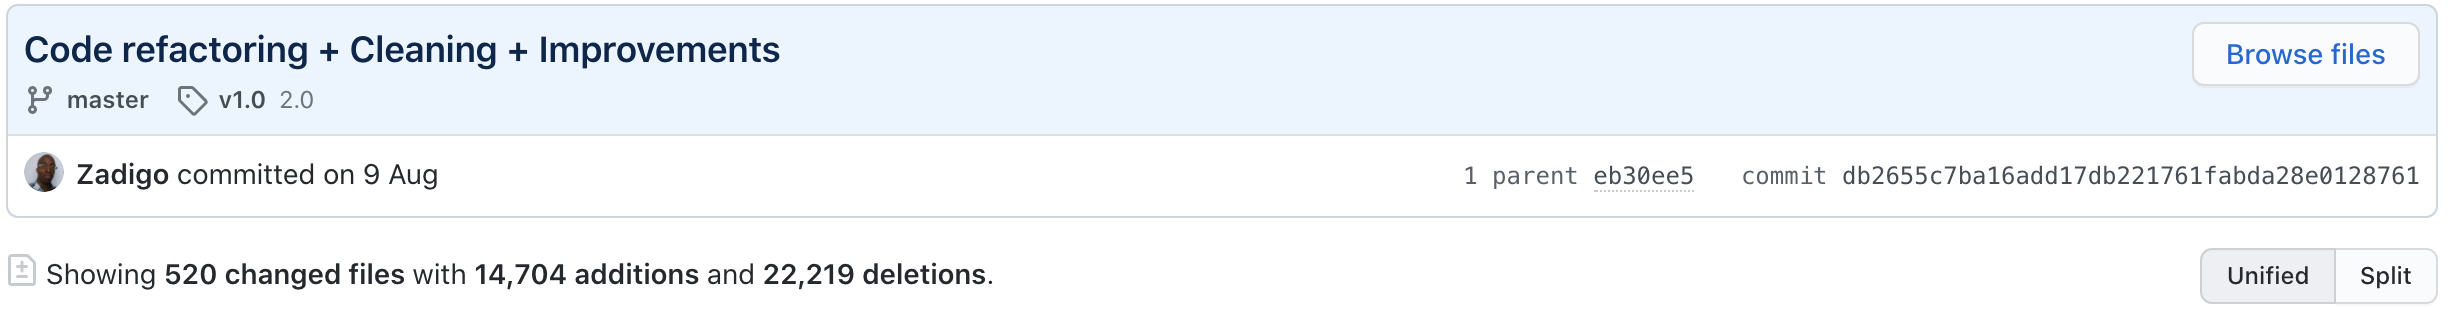
\includegraphics[width=1\linewidth]{img/ML/commit_messages/screen_1.png}
    \end{subfigure}
    \begin{subfigure}{\textwidth}
        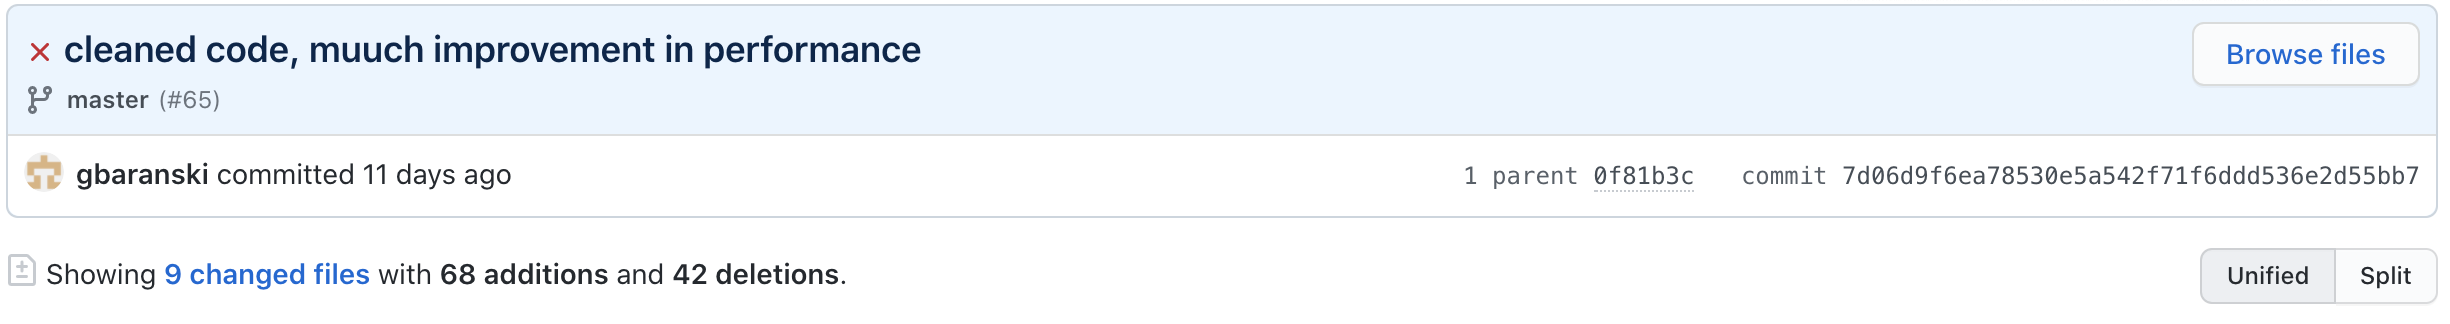
\includegraphics[width=1\linewidth]{img/ML/commit_messages/screen_2.png}
    \end{subfigure}
    \begin{subfigure}{\textwidth}
        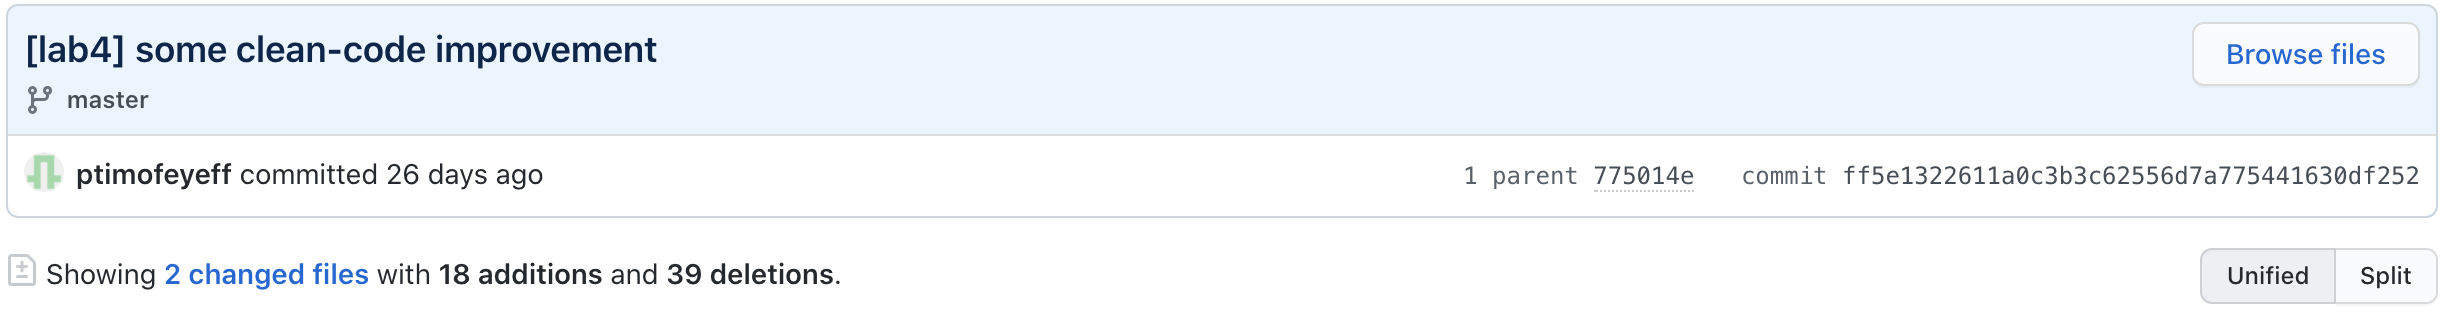
\includegraphics[width=1\linewidth]{img/ML/commit_messages/screen_3.png}
    \end{subfigure}
    \caption[Example commit messages that underline the inconsistency in commit message naming.]
    {Example commit messages from different repositories. Those examples highlight (1) the missing naming convention, (2) inclusion of additional performance improvements, and (3) several edits in multiple files~\cite{pendenque_code_2020, baranski_cleaned_2020, timofeev_lab4_2020}. Those commits were found by searching GitHub for \enquote{clean code improvements} and filtering for results of type commits and language Python. }
    \label{fig:commit_messages}
\end{figure}


\subparagraph{Solution 3:}
Since Python code is available in abundance in the form of open-source projects, it is possible to manually label source code that violates clean code rules. 
For the following reasons, we dismissed this approach:
\begin{enumerate}
    \item Curating a hand-labelled dataset is a time-consuming task. 
    \item Manual labelling does not ensure correct labelling. A human can make mistakes or can subjectively misinterpret chaotic code as clean code. The quality of the dataset could suffer and limit the machine learning models performance.
\end{enumerate}

\subparagraph{Solution 4:}
Given any amount of Python files, we could use the analysis plugins from \Cref{sec:analysis_plugins} to reliably detect violations of the corresponding rule. Based on this labelled data, we could train the classifier to detect those rule violations. The analysis plugins only cover rule violations of basic level of complexity, so the trained classifier could only detect rule violations that could also be detected by a basic checker. However, if there would be a labelled dataset for more complex clean code rules, we could transfer the findings to these more complex rules. 

We choose this solution to solve the dataset problem and train classifier. We can automatically generate labelled data with correct and consistent labels. Furthermore, this solution allows for scaling the dataset size if necessary. We will use the analysis plugins to label the three problem types: \texttt{RETURN NONE} (RN), \texttt{CONDITION COMPARISON SIMPLE} (CCS) and \texttt{CONDITION COMPARISON} (CC). However, this implies that we train the classifier to detect rule violations that could be detected by simple analysis plugins. If a labelled dataset for rules with a high level of complexity becomes available, we hope to transfer our findings to those rule violations as well.
In \hyperref[rq:3]{RQ3}, we will then test those classifiers on unseen variations of the rule violations to test the generalisation of the models. This gives an outlook on the transfer the training on rules with a high-level complexity by simulating a hand-labelled training set that is limited in problem variations.

\paragraph{Imbalanced Dataset}\label{sec:inbalanced_dataset}
A second challenge is a major imbalance between the samples labelled as problematic code and clean code. For the three different problem types, RN, CCS, and CC, the class distribution is shown in \Cref{tab:class_distribution_in_dataset}. The imbalance is especially severe for the RN type since only two out of 1000 samples contain the rule violation. For the CCS and CC type, the class are slightly more balanced with 26 and 49 samples with rule violations out of 1000.

\begin{table}[b]
    \centering
    \begin{tabular}{@{}crrr@{}}
    \toprule
    Label  & \multicolumn{1}{c}{RN} & \multicolumn{1}{c}{CCS} & \multicolumn{1}{c}{CC} \\ \midrule
    0 & 99.79\%     & 97.36\%          & 95.14\%              \\
    1 & 0.21\%      & 2.64\%           & 4.86\%               \\ \bottomrule
    \end{tabular}
    \caption[Class distribution for the dataset.]{Class distribution for the dataset. Label [0] represents clean code and label [1] marks problematic code of the corresponding category.}
    \label{tab:class_distribution_in_dataset}
    \end{table}

We combined the following solutions:
\subparagraph{Solution 1:}
Due to the imbalance, we do not choose accuracy as a suitable evaluation metric, since classifying all samples as clean code would result in an accuracy of 99.79\% for the RN problem type. Instead, we use precision and recall as metrics, with an f1 score as a single, weighted metric. More details about the metrics are in \Cref{par:approach}.

\subparagraph{Solution 2:}
We will apply undersampling and oversampling techniques on the data and evaluate the difference in model performance. Undersampling removes random samples from the majority class and thus balance class labels. Oversampling replicates random samples from the minority class to balance class labels while also increasing the overall amount of data. This technique is only used for the training data since it would distort the evaluation results when applied to test data as well.

\subparagraph{Solution 3:}
Our approach of training different classifier is a solution to the data imbalance since different classifiers have a different sensitivity to data balance. 

\paragraph{SVM quadratic complexity in training}\label{sec:svm_quadratic_complexity}
The implementation of the support vector machine has a quadratic time complexity on the number of training data~\cite{abdiansah_time_2015}. Consequently, the training takes much time and the oversampling strategy worsen the training time further since it introduces more samples.
\subparagraph{Solution:}
We reduce the number of experiments with SVM and just evaluate some simple cases for baseline performance. 


\subsection{Dataset}\label{chap:clean_code_classification_dataset}
The source of our dataset are open-source Python projects on GitHub. We queried the top starred Python repositories and handselected 18 repositories. Although most top stared repositories are data science frameworks, we explicitly choose projects from other domains such as web server, automation and containerisation. In \Cref{tab:repos_domains}, we list all projects with the corresponding domain.
\begin{table}[h]
    \centering
    \csvautobooktabular{tables/dataset_category.csv}
    \caption{Open-source repositories we used in our dataset and their corresponding domain. }
    \label{tab:repos_domains}
\end{table}

A script downloaded all projects in their main branch with the current head. See \Cref{tab:repos_hashes} for the corresponding git hashes. Afterwards, we removed all non-python files. 
Next, we uniformly sampled 20\% of all files and separated those into a holdout set for testing and the code manipulation in \hyperref[rq:3]{RQ3}. Additionally, we perform our train/test split on the file level and not on the sample level. We describe the reason for the file level split later in \Cref{sec:train_test_split}.

We ensured to have similar data and label distribution on all data sets. \Cref{tab:general_data_distribution} shows general and problem-specific metrics on file level for the train, test and holdout set. The problem-specific metrics are collected after processing the code files as described in \Cref{sec:data_encoding}. We define the metrics as follows:

We calculate the \textit{average lines of code per file} for $n$ files with $l_i$ as the lines of code for file $i$ with the following equation:
\[
  \textit{average LOC per File} = \frac{\sum_{i=0}^n{l_i}}{n}  
\]
For the \textit{proportion of lines of code containing a problem}, we assume one line contains the problem. Therefore, we define this metric for $n$ files with $l_i$ lines of code for the $i$th file and $p_i$ problems in the $i$th file as follows:
\[
    \textit{LOCs containing problem} = \frac{\sum_{i=0}^n{p_i}}{\sum_{i=0}^n{l_i}}
\]
Last, we calculate the number of problems per file for $n$ files and $p_i$ problems in the $i$th file as:
\[
    \textit{Problems per File} = \frac{\sum_{i=0}^n{p_i}}{n}
\]

The most important metrics for the data distribution is the proportion of lines of code containing the problem type and the average number of problems per file. For lines of code containing the problem type, we observe a maximal difference of 0.02 percentage points between the datasets for the RN problem type, 0.11 percentage points for CCS and 0.13 percentage points for the CC problem type. This directly translates into the class distribution as shown in \Cref{tab:class_distribution} with a maximal difference 0.06, 0.26 and 0.31 percentage points for the three problem types.
The number of problems per file is lower in the test set for the CCS and CC problem type. Nevertheless, the size of a file may vary, and thus the number of problems per file may vary too. Since the lines of code containing the problem and the class frequencies are comparable, our datasets have a comparable data distribution over the different dataset splits.

TODO per-project analysis table in attachments?

\begin{table}[]
    \tabcolsep=0.11cm
    \begin{tabularx}{\textwidth}{@{}llXXX@{}}
        \toprule
    %\cmidrule(l){2-4}
    \multirow{4}{*}{}                            & Metric                  & Train & Test & Holdout \\ \cmidrule(l){2-5} 
                                                 & Lines of Code           & 2,530,455 & 246,813 & 671,554 \\
                                                 & Number of Files         & 13,330  &  1,481 & 3,702   \\
                                                 & average LOC per File    & 189.83  & 166.65  & 181.40     \\ \midrule
    \multirow{2}{*}{Return None}                 & LOCs containing problem & 0.07\%  &  0.09\% & 0.08\%  \\
                                                 & Problems per File       & 0.14    & 0.15  & 0.14    \\ \midrule
    \multirow{2}{*}{Condition Comparison Simple} & LOCs containing problem & 1.29\%  &  1.21\%  & 1.32\%  \\
                                                 & Problems per File       & 2.44    & 2.02 & 2.4    \\ \midrule
    \multirow{2}{*}{Condition Comparison}        & LOCs containing problem & 2.34\%  & 2.31\%  & 2.44\%  \\
                                                 & Problems per File       & 4.44    & 3.85  & 4.42    \\ \bottomrule
    \end{tabularx}
    \caption{General and problem specific metrics for the train, test and holdout set.}
    \label{tab:general_data_distribution}
\end{table}

\begin{table}[]
    \begin{tabularx}{\textwidth}{@{}lXXXX@{}}
    \toprule
    Problem Type                                 & Label& Train & Test & Holdout \\ \midrule 
    \multirow{2}{*}{Return None}                 & [0] & 99.79\%  & 99.73\% & 99.78\%  \\
                                                 & [1] & 0.21\%   & 0.27\%  & 0.22\%    \\ \midrule
    \multirow{2}{*}{Condition Comparison Simple} & [0] & 97.34\%   &  97.49\%  & 97.23\%  \\
                                                 & [1] & 2.66\%   & 2.51\% & 2.77\%    \\ \midrule
    \multirow{2}{*}{Condition Comparison}        & [0] & 95.13\%  & 95.21\%  & 94.9\%  \\
                                                 & [1] & 4.87\%   & 4.79\%  & 5.1\%    \\ \bottomrule
    \end{tabularx}
    \caption{Class frequencies for all problem types on the train, test and holdout set. We observe a compareable class distribution amoung the datasets for each problem type.}
    \label{tab:class_distribution}
\end{table}


\begin{figure}
    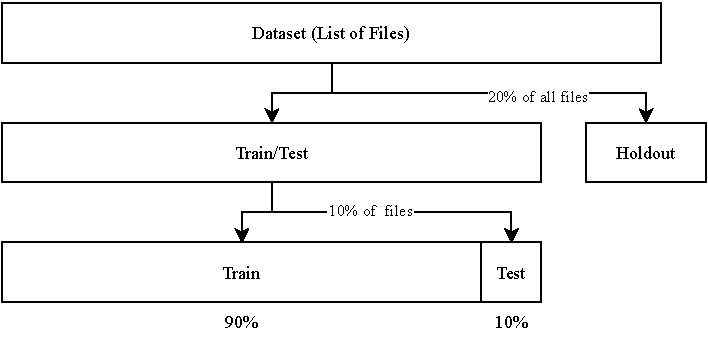
\includegraphics[width=1\textwidth]{img/ML/Data_split.pdf}
    \caption{Split of the dataset. First, 20\% of all files are seperated into a holdout set for later testing. The remainding 80\% of the files are split into 90\% training and 10\% test data. }
    \label{fig:data_split}
\end{figure}

\subsection{Processing}
For the processing steps, we create a pipeline with the d6tflow framework\footnote{\url{https://github.com/d6t/d6tflow}}. Each processing step is a task that stores its results depending on the parameter configuration in a pickle file. This allows to define a pipeline once and run it with different parameter combinations. The scheduler automatically determines what tasks to run and what task outputs are already stored. Consequently, running the pipeline is more efficient and repeatable.

The processing pipeline consists of tasks to read the files into a data structure, to process source code and find the problems, to create a vocab dictionary, to convert the data into labelled samples. In \Cref{fig:pipeline_rq2}, we provide a schematic representation of the pipeline.

\begin{figure}
    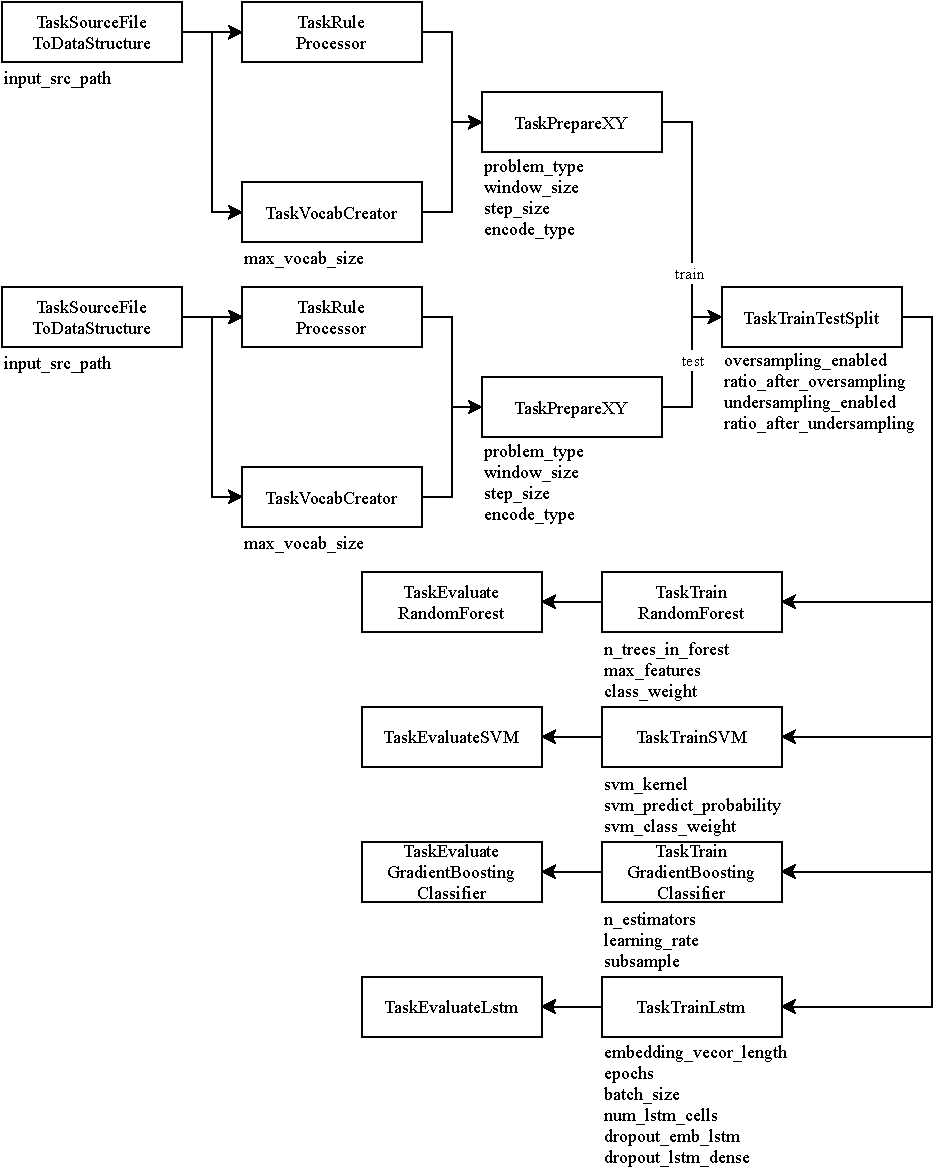
\includegraphics[width=1\textwidth]{img/ML/Pipeline_RQ2.pdf}
    \caption[Schematic representation of the pipeline to train and test models.]{Schematic representation of the pipeline for \hyperref[rq:2]{RQ2} to train and test models with configurable parameters. First, the pipeline reads the source code into memory, extract the vocabulary (\texttt{TaskVocabCreator}) and identify all problem types (\texttt{TaskRuleProcessor}). It the converts the code of dynamic length into fixed-size samples (\texttt{TaskPrepareXY}). This sub-pipeline runs seperate for the train and test set. In \texttt{TaskTrainTestSplit}, both datasets are combined and over- or undersampling is applied to the train set. The train set is used to train different classifiers wheras the train and test set are used for evaluation.}
    \label{fig:pipeline_rq2}
\end{figure}


\subsubsection{Files into Internal Data Structure}
First, a scanner walks recursively over all subdirectories of the input folder to find all files. If the file has a \texttt{.py} extension, its file path and the file content will be stored in a dictionary. The dictionaries for all files are collected into a list. 
Reading all files into main memory increases the performance for downstream tasks since main memory access is faster than disk access. Although the size of the system's main memory limits the dataset size, a file contains text and is just several kilobytes in size. The train dataset with 13,330 files is 86.47MB in accumulated file size.

\subsubsection{Problem Detection}\label{sec:problem_detection}
As a next step, the analysis plugins from the CCAP (see \Cref{sec:analysis_plugins}) process every file and store the line number along with the problem type (RN, CCS, or CC). As a result, for every file, a list of problematic line numbers and the corresponding type is available for further processing. 

\subsubsection{Data Encoding}\label{sec:data_encoding}
The data encoding step transforms the internal data representation into the input vector $x$ and output vector $y$. One $(x,y)$ pair describes a sample with input and ground-truth label. The transformation happens in the following multi-stage process:
\paragraph{Fixed Length Sequence}
The length of the source code is dynamic, whereas the input size of our models is fixed. Therefore, the character stream of variable length has to be transformed into a token stream of fixed size. 
To extract meaningful tokens from the character stream, we use the Python tokenizer from its standard library. The tokenizer separates the character stream based on the python syntax definition into tokens. All tokens contain a token type (like a name or operator token), the corresponding characters in the source code and a start and end position (line and column number). Afterwards, the token stream is divided into a fixed size token sequence using a sliding window approach. The step and window size are configurable, and we use a window size of 20 and a step size of 3 in our experiments. The sliding window operation is part of the \texttt{TaskPrepareXY} step in the pipeline.
\paragraph{Vocabulary Creation}
In order to feed the textual token values into a model, we need to transform it into a numeric representation. Since our token values can be the entire value of a string literal, we can not encode every single token value into a number. We create a vocabulary with a limited size that contains the most common token values and a numerical representation for all other values.
Therefore, the occurrence of each token value is counted and sorted based on their frequency. To ignore potential capitalisation mismatches, all token values are lower-case. The overall size of the vocabulary is configurable. If the size is smaller than the size of the distinct token value set, the least common token values will be replaced by an unknown token. The unknown token has a numeric representation one bigger than the vocabulary size. We found that using a vocabulary size of 100,000 results in an acceptably low 3.9\% of token values being unknown. In our pipeline, the task \texttt{TaskVocabCreator} creates the vocabulary.
\paragraph{Index-Based Encoding}
The textual token values are encoded with an Index-Based encoding. The most common token values have a numerical representation based on their index in a vocabulary (created with all token values of the train data). Optional, the type of each token is encoded by its numerical representation in the standard library (see \Cref{fig:tokenizer_types}). The type and value encodings are then combined alternating in a final encoding vector $x_i$ for every sample $i$.
\paragraph{Label Extraction}
With the internal representation, the ground truth is encoded as a line number. This representation has to be transformed in a label $y_i$ for the given input vector $x_i$ for sample $i$. Label 1 is assigned if the sample contains the given problem type. A sample contains a problem type if it contains all tokens from the problematic line. If the sample is missing a token of the problematic line at the beginning or end, the label is 0 for non-problematic code.
After the label extraction in the pipeline step \texttt{TaskPrepareXY}, we have a list of input vectors $x$ and a list of ground truth labels $y$. With this, we can train and test our models.

\subsubsection{Train/Test Split}\label{sec:train_test_split}
In \Cref{chap:clean_code_classification_dataset}, we described to create a train, test and holdout dataset by file-level separation and not by splitting the samples. The reason for this approach is our sliding window concept. Since we use the sliding window to convert source files with dynamic length into fixed-length token sample samples, we may have one problematic code pattern in multiple samples. The difference would be in the location inside the sample and the surrounding tokens, whereas the pattern remains the same.
If we would do a train/test split on a sample level, we may introduce samples covering one problematic pattern in both datasets. \Cref{fig:encoding_sliding_window} illustrates multiple windows covering one sample. 

This unclean separation would diminish the validity of metrics calculated from the test and holdout dataset. Therefore, we split on file level and perform the previous preprocessing separately for training and test dataset. Only the vocabulary generation happens on the training file for both processing steps. In \texttt{TaskPrepareXY} in the pipeline, we then merge those two pipelines for training and testing (see \Cref{fig:pipeline_rq2}).
\begin{figure}
    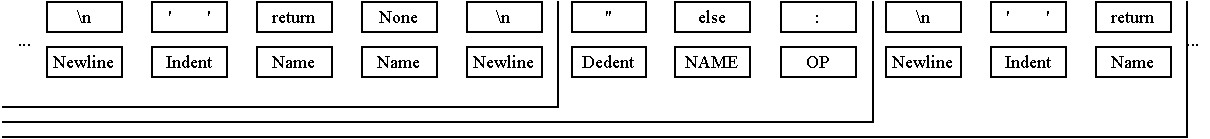
\includegraphics[width=1\textwidth]{img/ML/encoding_sliding_window_problem.pdf}
    \caption[Sliding window approach on source code containing a problematic \texttt{return None}]{Sliding window approach on source code containing a problematic \texttt{return None}. Multiple windows will contain the problematic sample. Consequently, we can not split on a sample level, since the same problem would be in the train and test set. Instead, we split on file level to have a clean separation between the datasets.}
    \label{fig:encoding_sliding_window}
\end{figure}

\subsubsection{Code Manipulation}\label{sec:approach_code_manipulation}
In research question \hyperref[rq:3]{RQ3}, we evaluate the models' generalisation to detect similar pattern the model was not trained on. Therefore, we manipulate the code that it is still a rule violation, but the original analysis plugins would not spot them. The pipeline for code manipulation differs from the pipeline for RQ2 by an additional code manipulation task and removal of the training step (see \Cref{fig:pipeline_RQ3}).

\begin{figure}
    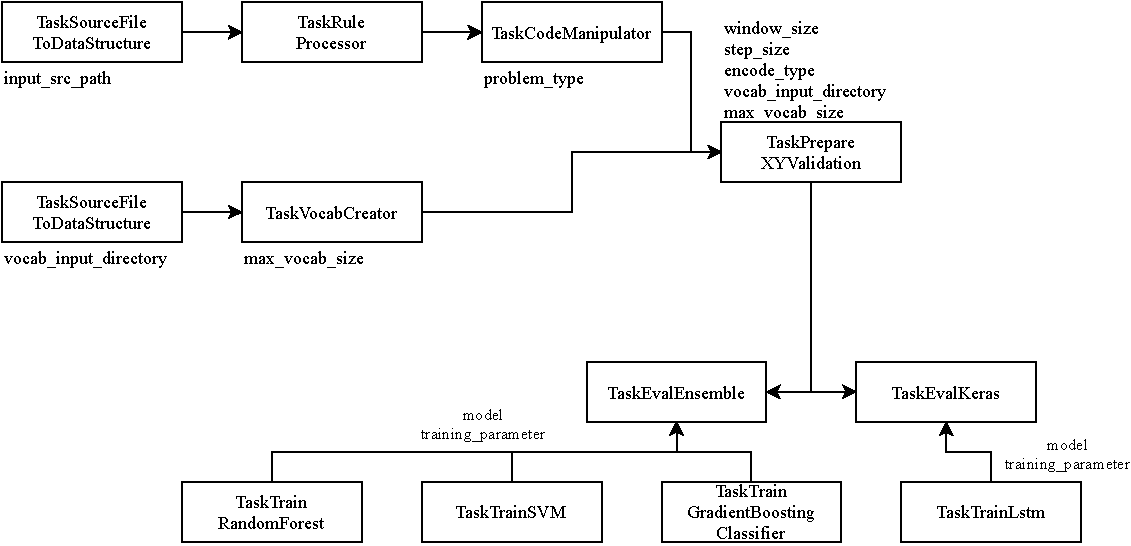
\includegraphics[width=1\textwidth]{img/ML/Pipeline_RQ3.pdf}
    \caption[Pipeline for code manipulation and evaluation.]{Pipeline for code manipulation and evaluation. The prerpocessing part is like in \Cref{fig:pipeline_rq2} but with an additional \textit{TaskCodeManipulator} to manipulate the code as described in \Cref{sec:approach_code_manipulation}. The random forest classifier, svm and gradient boosting classifier require different evaluation code as the LSTM, so two \textit{TaskEval*} are used. }
    \label{fig:pipeline_RQ3}
\end{figure}


\paragraph{Return None}\label{par:manipulation_return_none}
For the RN problem type, we manipulate the code to have an inline if statement that only returns \texttt{None} in one branch. Therefore, a function may still return None, but the analysis plugin would not detect it. \Cref{lst:return_none_modified} shows an example for this case. Although a modification of the analysis plugin could cover the variations as well, we want to see how well machine learning models could perform on this task.

To modify the original code, we use the preprocessed code with problems detected as in \Cref{sec:problem_detection}. For every source code line containing the RN problem, we use regular expressions to replace the \textit{return None} with a variation as seen in \Cref{lst:return_none_modified}. 

The subsequent data encoding step is similar to the one for model training, although this modified samples will only be used during evaluation.

\begin{minipage}[c]{\linewidth}
\begin{lstlisting}[language=Python, label=lst:return_none_modified, caption={Samples for returning None. The analysis plugin would flag the first return; the second and third return are modified variations that would be ignored by the analysis plugin. The performance of the machine learning models on detecting the latter will be evaluated.}]
def f(a,b):
    #detected by the analysis plugin
    return None 

    #not detected by the analysis plugin
    return None if a < b else b 

    #not detected by the analysis plugin
    return a if a < b else None \end{lstlisting}
\end{minipage}
\paragraph{Condition Comparison}\label{par:manipulation_condition_comparison}
We want to test the generalisation of the model trained on the CCS types by evaluating on the labelled data for the CC type. 
Since the dataset for the CC type includes the CCS subset, we manipulate the CC dataset to only contain samples the CCS was not trained on. The sample in \Cref{lst:conidtion_comparison_modified} shows the manipulation to ensure that all CC problems were not part of the CCS training set. The implementation uses a similar regular expression approach as described in \Cref{par:manipulation_return_none}

\begin{lstlisting}[language=Python, label=lst:conidtion_comparison_modified, caption={Sample statements for the differnce between the two analysis plugins CC and CCS.  }]
    def f(a,b):
    #detected by CONDITION COMPARISON SIMPLE
    #detected by CONDITION COMPARISON
    if a < b:
        pass 

    #manipulated
    #not detected by CONDITION COMPARISON SIMPLE
    #detected by CONDITION COMPARISON
    if not a < b:
        pass 

    #manipulated
    #not detected by CONDITION COMPARISON SIMPLE
    #detected by CONDITION COMPARISON
    if is_smaller(a,b) and b < c::
        pass \end{lstlisting}

\subsection{Models}
Classifying code samples is a binary classification problem since we consider each problem type as a separate classification task. We train and evaluate a random forest classifier, a support-vector machine-based classifier, a gradient boosting classifier and a neural network with LSTM cells.

\paragraph{Random Forest}
We use a random forest classifier with 100 decision trees to perform the binary classification. Additional to over- and undersampling, we experiment with an automatic class weighting inverse proportional to class frequency. The other hyperparameter follows the default implementation of the scikit-learn library: The quality measure of a split follows the Gini function, the tree depth is unlimited and the number of features to consider for each split is the square-root of the number of features overall. We use the implementation in the scikit-learn library in version 0.23.2~\cite{scikit-learn}.
\paragraph{Support Vector Machine}
We use the support-vector classification from the scikit-learn library~\cite{scikit-learn}. As a kernel function, we choose the radial basis function for a performance baseline. Additionally, we try the class weighting inverse proportional to the class frequency to combat the imbalanced dataset.
\paragraph{Gradient Boosting Classifier}
For gradient boosting classifier, we mainly vary the number of boosting steps and the learning rate. Furthermore, we experiment with stochastic gradient boosting by setting the subsample parameter to 0.4 and 0.7. Other hyperparameter settings follow the default value of the scikit-learn library~\cite{scikit-learn}.
\paragraph{Neural Networks with LSTM Cells}
Our neural network consists of five layers (see \Cref{lst:lstm}). First, we use an embedding layer with an embedding size of 32. The input is the Index-Based encoded samples without type encoding. This layer is trained end-to-end with the complete network on the trainings-data. Furthermore, this layer covers most trainable parameters of the model. As a hidden layer, we use 10 LSTM cells with a prior and posterior dropout layer with a default 0.2 dropout. To perform binary classification, our model ends with a dense mapping onto a single neuron. The binary result is determined based on a 0.5 threshold for the output of the last neuron.

We vary the hyperparameters for batch size, number of epochs, embedding size and number of LSTM cells. For implementation, we use Keras in version 2.4.3~\cite{chollet2015keras}.

\begin{lstlisting}[label=lst:lstm, caption={Summary of our LSTM network. We use an embedding layer of size 32, 10 LSTM cells, a dropout layer before and after the LSTM layer with a default dropout ratio of 0.2 and a dense mapping to a single output neuron for binary classification with a threshold of 0.5.}]
Layer (type)                 Output Shape              Param #
============================================
embedding (Embedding)        (None, 20, 32)            3200064
__________________________
dropout (Dropout)            (None, 20, 32)            0
__________________________
lstm (LSTM)                  (None, 10)                1720
__________________________
dropout_1 (Dropout)          (None, 10)                0
__________________________
dense (Dense)                (None, 1)                 11
============================================
Total params: 3,201,795
Trainable params: 3,201,795
Non-trainable params: 0\end{lstlisting}